\documentclass[12pt,a4paper]{article}
\usepackage[utf8x]{inputenc}
\usepackage{ucs}
\usepackage{amsmath}
\usepackage{amsfonts}
\usepackage{amssymb}
\usepackage{graphicx}
\usepackage{listings}
\usepackage[left=2cm,right=2cm,top=2cm,bottom=2cm]{geometry}

\usepackage{natbib}
\bibpunct{[}{]}{,}{n}{}{;}

\usepackage[pdftex,pagebackref]{hyperref}
    \usepackage{natbib}
    \hypersetup{colorlinks,linktocpage=true}
\renewcommand{\backrefpagesname}{ \protect\\  \textit{Cited on
page(s):}~}
\renewcommand{\backref}{\backrefpagesname}

\author{Gergely Imreh}
\title{LabWeather}
\date{2013-03-21, v1}
\begin{document}
\maketitle

The purpose of the laboratory weather monitoring circuit was to double-check the air-conditioning system, and provide a quick overview to the (in)stability of the lab humidity and temperature.

\tableofcontents

\section{Sensors}

\subsection{Humidity sensor}

The humidity sensor used is a general CM-R resistive humidity sensor \footnote{CM-R spec sheet: \url{http://file.yizimg.com/3381/20061221103057890280486.pdf}}. Because of its design, it is not allowed to have any DC voltage across it. This could be achieved by driving it with AC voltage, or more reliably by decoupling with capacitors from the DC parts of the circuit

The current circuit is shown on Fig. \ref{fig:circuit}, part 1.

To measure the resistance of the sensor, the controller is driving it at 1kHz (square waves), and at fixed intervals (every 0.5 or 1 seconds) the square wave is stopped and a quick resistance measurement is made, then the square wave is resumed. Since the sensor is working continuously for months without apparent change in behaviour, this seems to be safe enough. Also, the measured values are consisted with other independent humidity measurements (HOBO U10\footnote{HOBO U10 product page: \url{http://www.onsetcomp.com/products/data-loggers/u10-003}}).

The humidity vs. resistance can be derived from the spec sheet, for recording purposes the current version is assuming $25\mathrm{^\circ C}$ temperature, which is close enough, $\approx \pm 5 \% $ error for our lab temperature range. Thus here it is
\begin{equation}
\mathrm{RH\%} =  2.76366367 \times (\log_{10} R) ^ 2 - 32.40924966 \times \log_{10}R + 102.93566686
\end{equation}
where the coefficients I got from fitting the spec sheet data.

Further improvement would be to rewire the sensor in an AC balanced bridge arrangement, but haven't had a chance to figure that one out.

\subsection{Temperature sensor}

Texas Instruments LM335 \footnote{LM335 product page: \url{http://www.ti.com/product/lm335}} in the simplest possible arrangement. It can be considered as a regular Zener-diode, with temperature dependent breakdown voltage, in this case $10\mathrm{mV}/\mathrm{K}$. Thus room temperature gives about $2.93\mathrm{V}$ across it.

The circuit is shown on Fig. \ref{fig:circuit}, part 2.

One problem is that the currently used Arduino's ADC has only 10bits over 0-5V, only being able to resolve about $0.5\mathrm{^\circ C}$, with quite a bit of noise. Thus the measured value needs to be averaged and filtered for practical use.

Further improvement is possibe to amplify the signal around the usual working voltage. Most likely it would be an op-amp in single-supply mode. Tried one such circuit with 10x amplification, the temperature resolution is better, but the measurement noise (measured by calculating the standard deviation) is only reduced by half. Thus this might not worth the extra effort.

\begin{figure}[ht!]
\centering
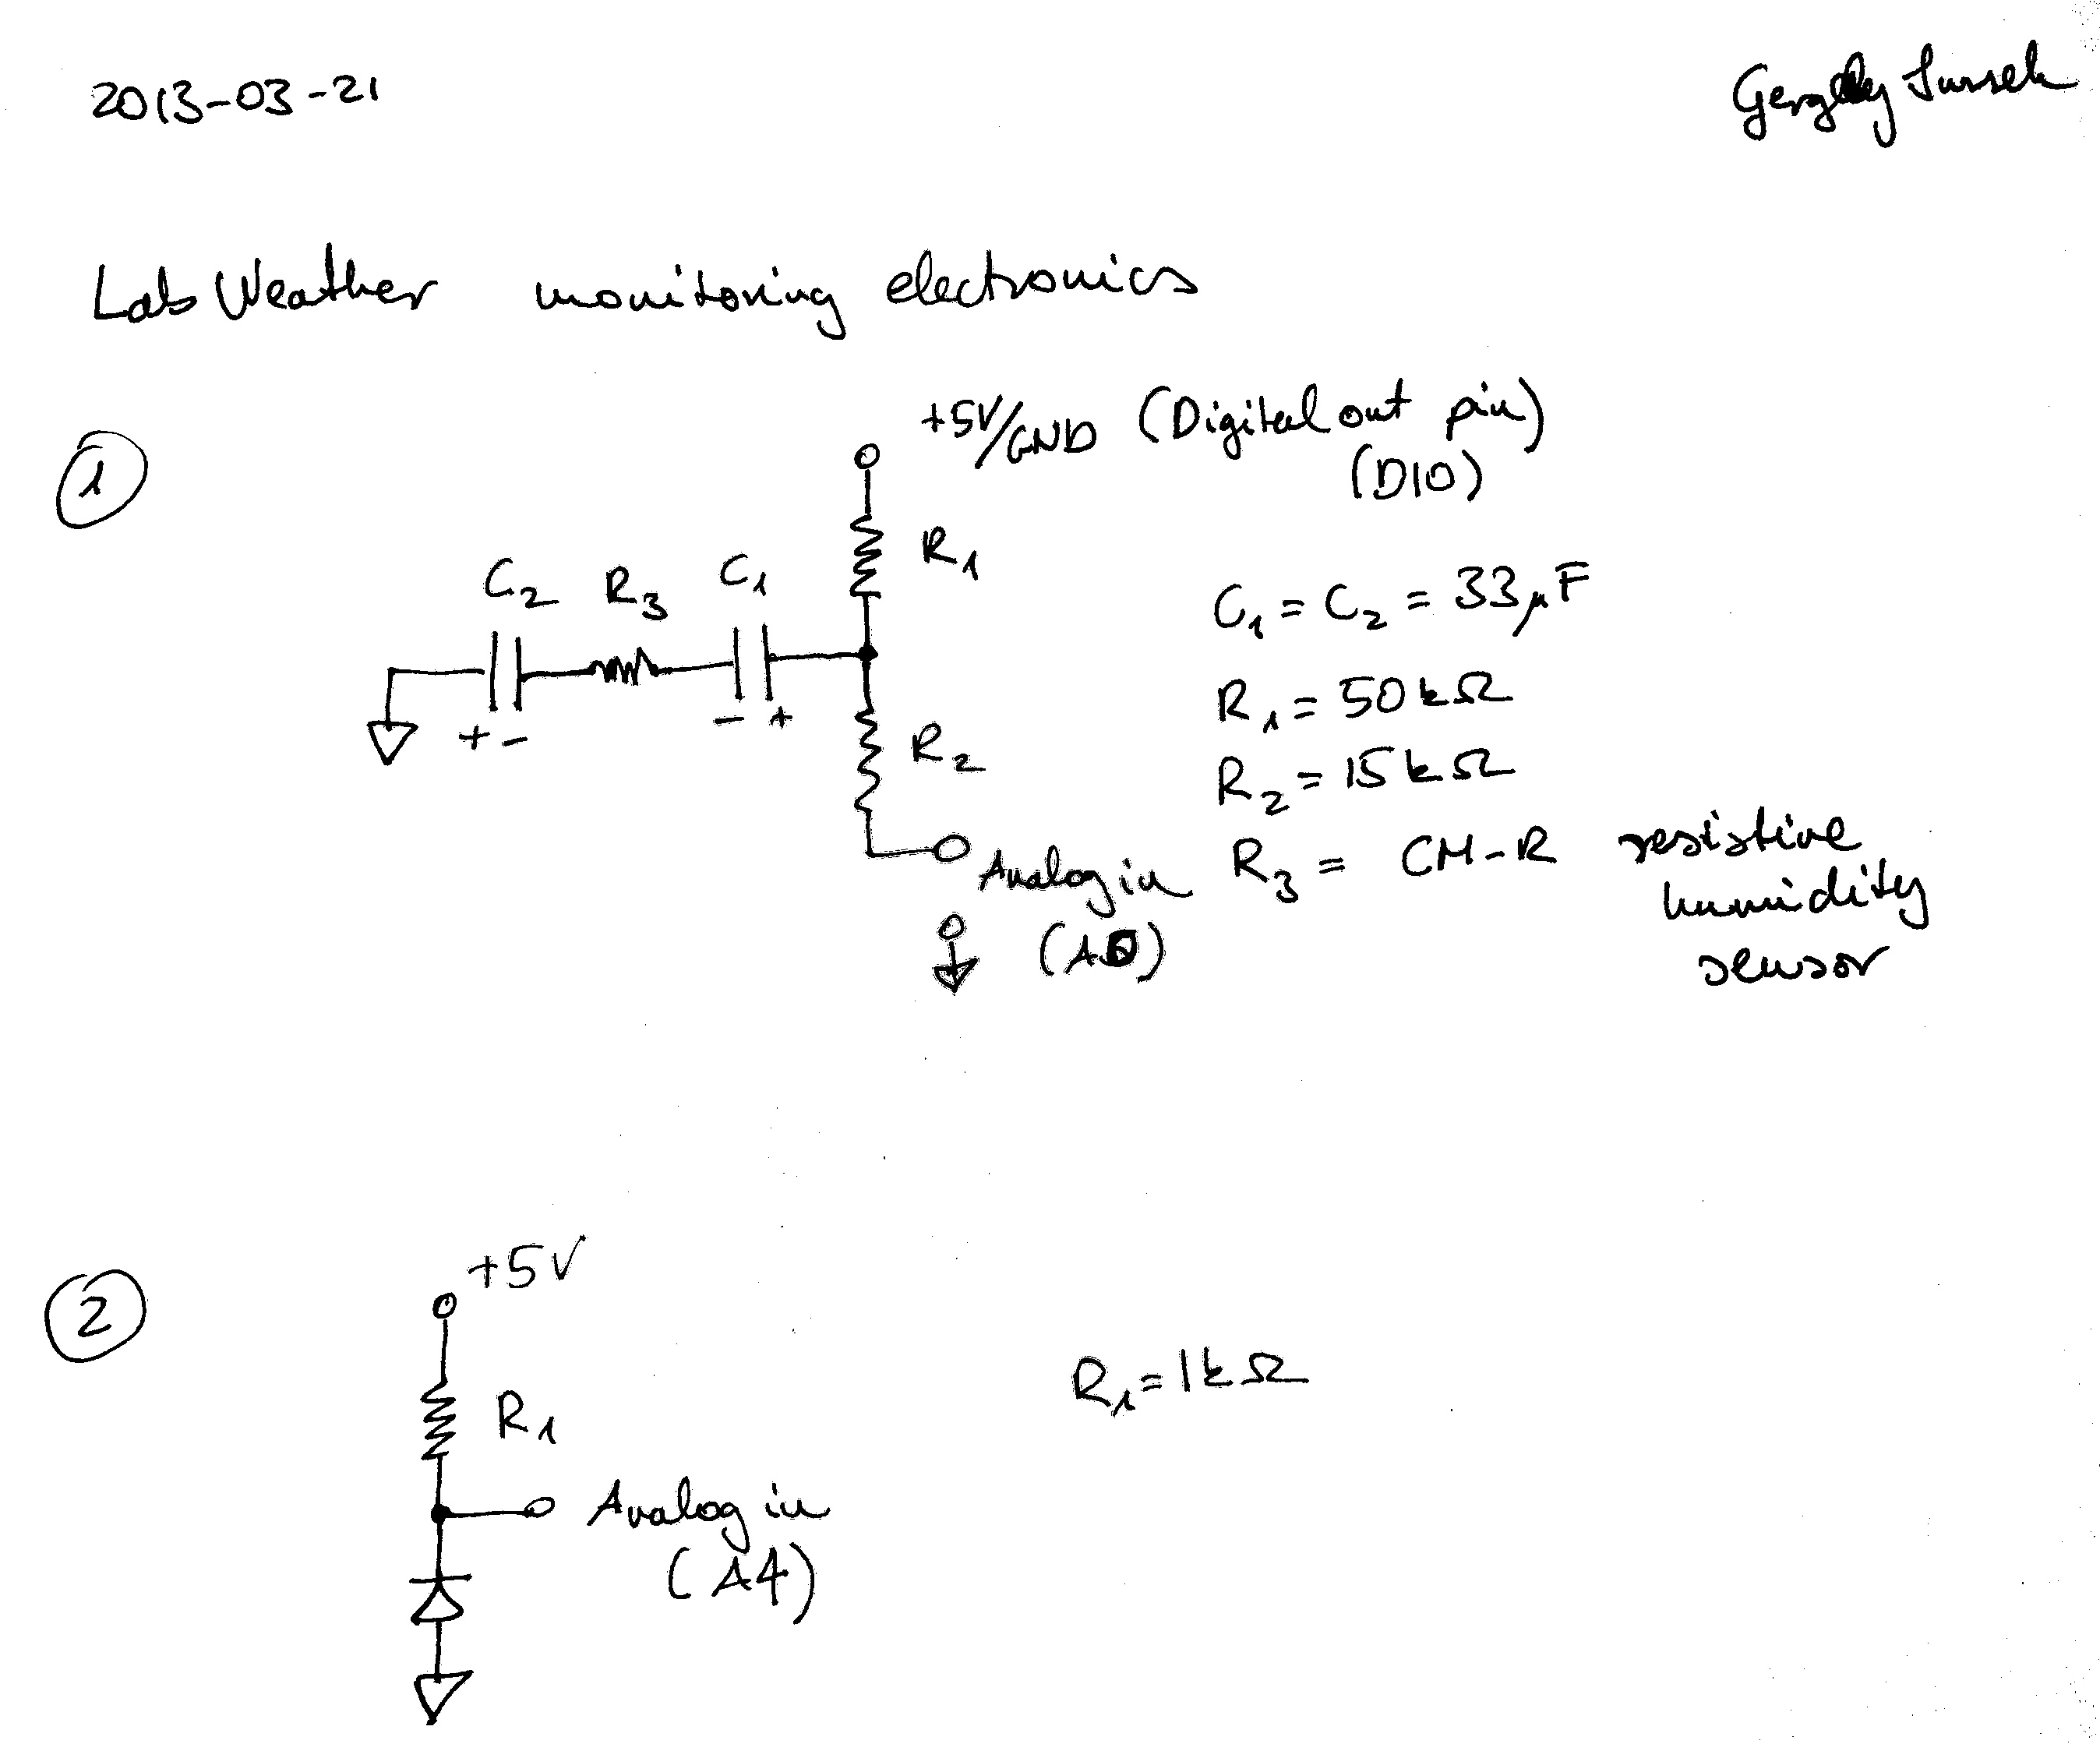
\includegraphics[width=140mm]{circuit.jpg}
\caption{The circuits for the lab weather monitoring setup}
\label{fig:circuit}
\end{figure}

\section{Data relay}

The resistance and voltage measurements for the humidity and currently done with an Arduino Diecimilla\footnote{Arduino Diecimilla product page: \url{http://arduino.cc/en/Main/ArduinoBoardDiecimila}}. It is obsolete product now, but any other Arduino should do the trick, and even could build a barebones kit with the Atmel328 microcontroller chips with not too much effort.

The current source code can be found on the net\footnote{Humidity sensor source code: \url{https://github.com/imrehg/weatherstation/tree/master/humidity1}}. When in doubt how to load that data onto the Arduino, consult it's Getting Started Guide\footnote{Arduino Getting Started: \url{http://arduino.cc/en/Guide/HomePage}}.

The Arduino sends the measured data to the computer via the attached USB cable.

\begin{figure}[ht!]
\centering
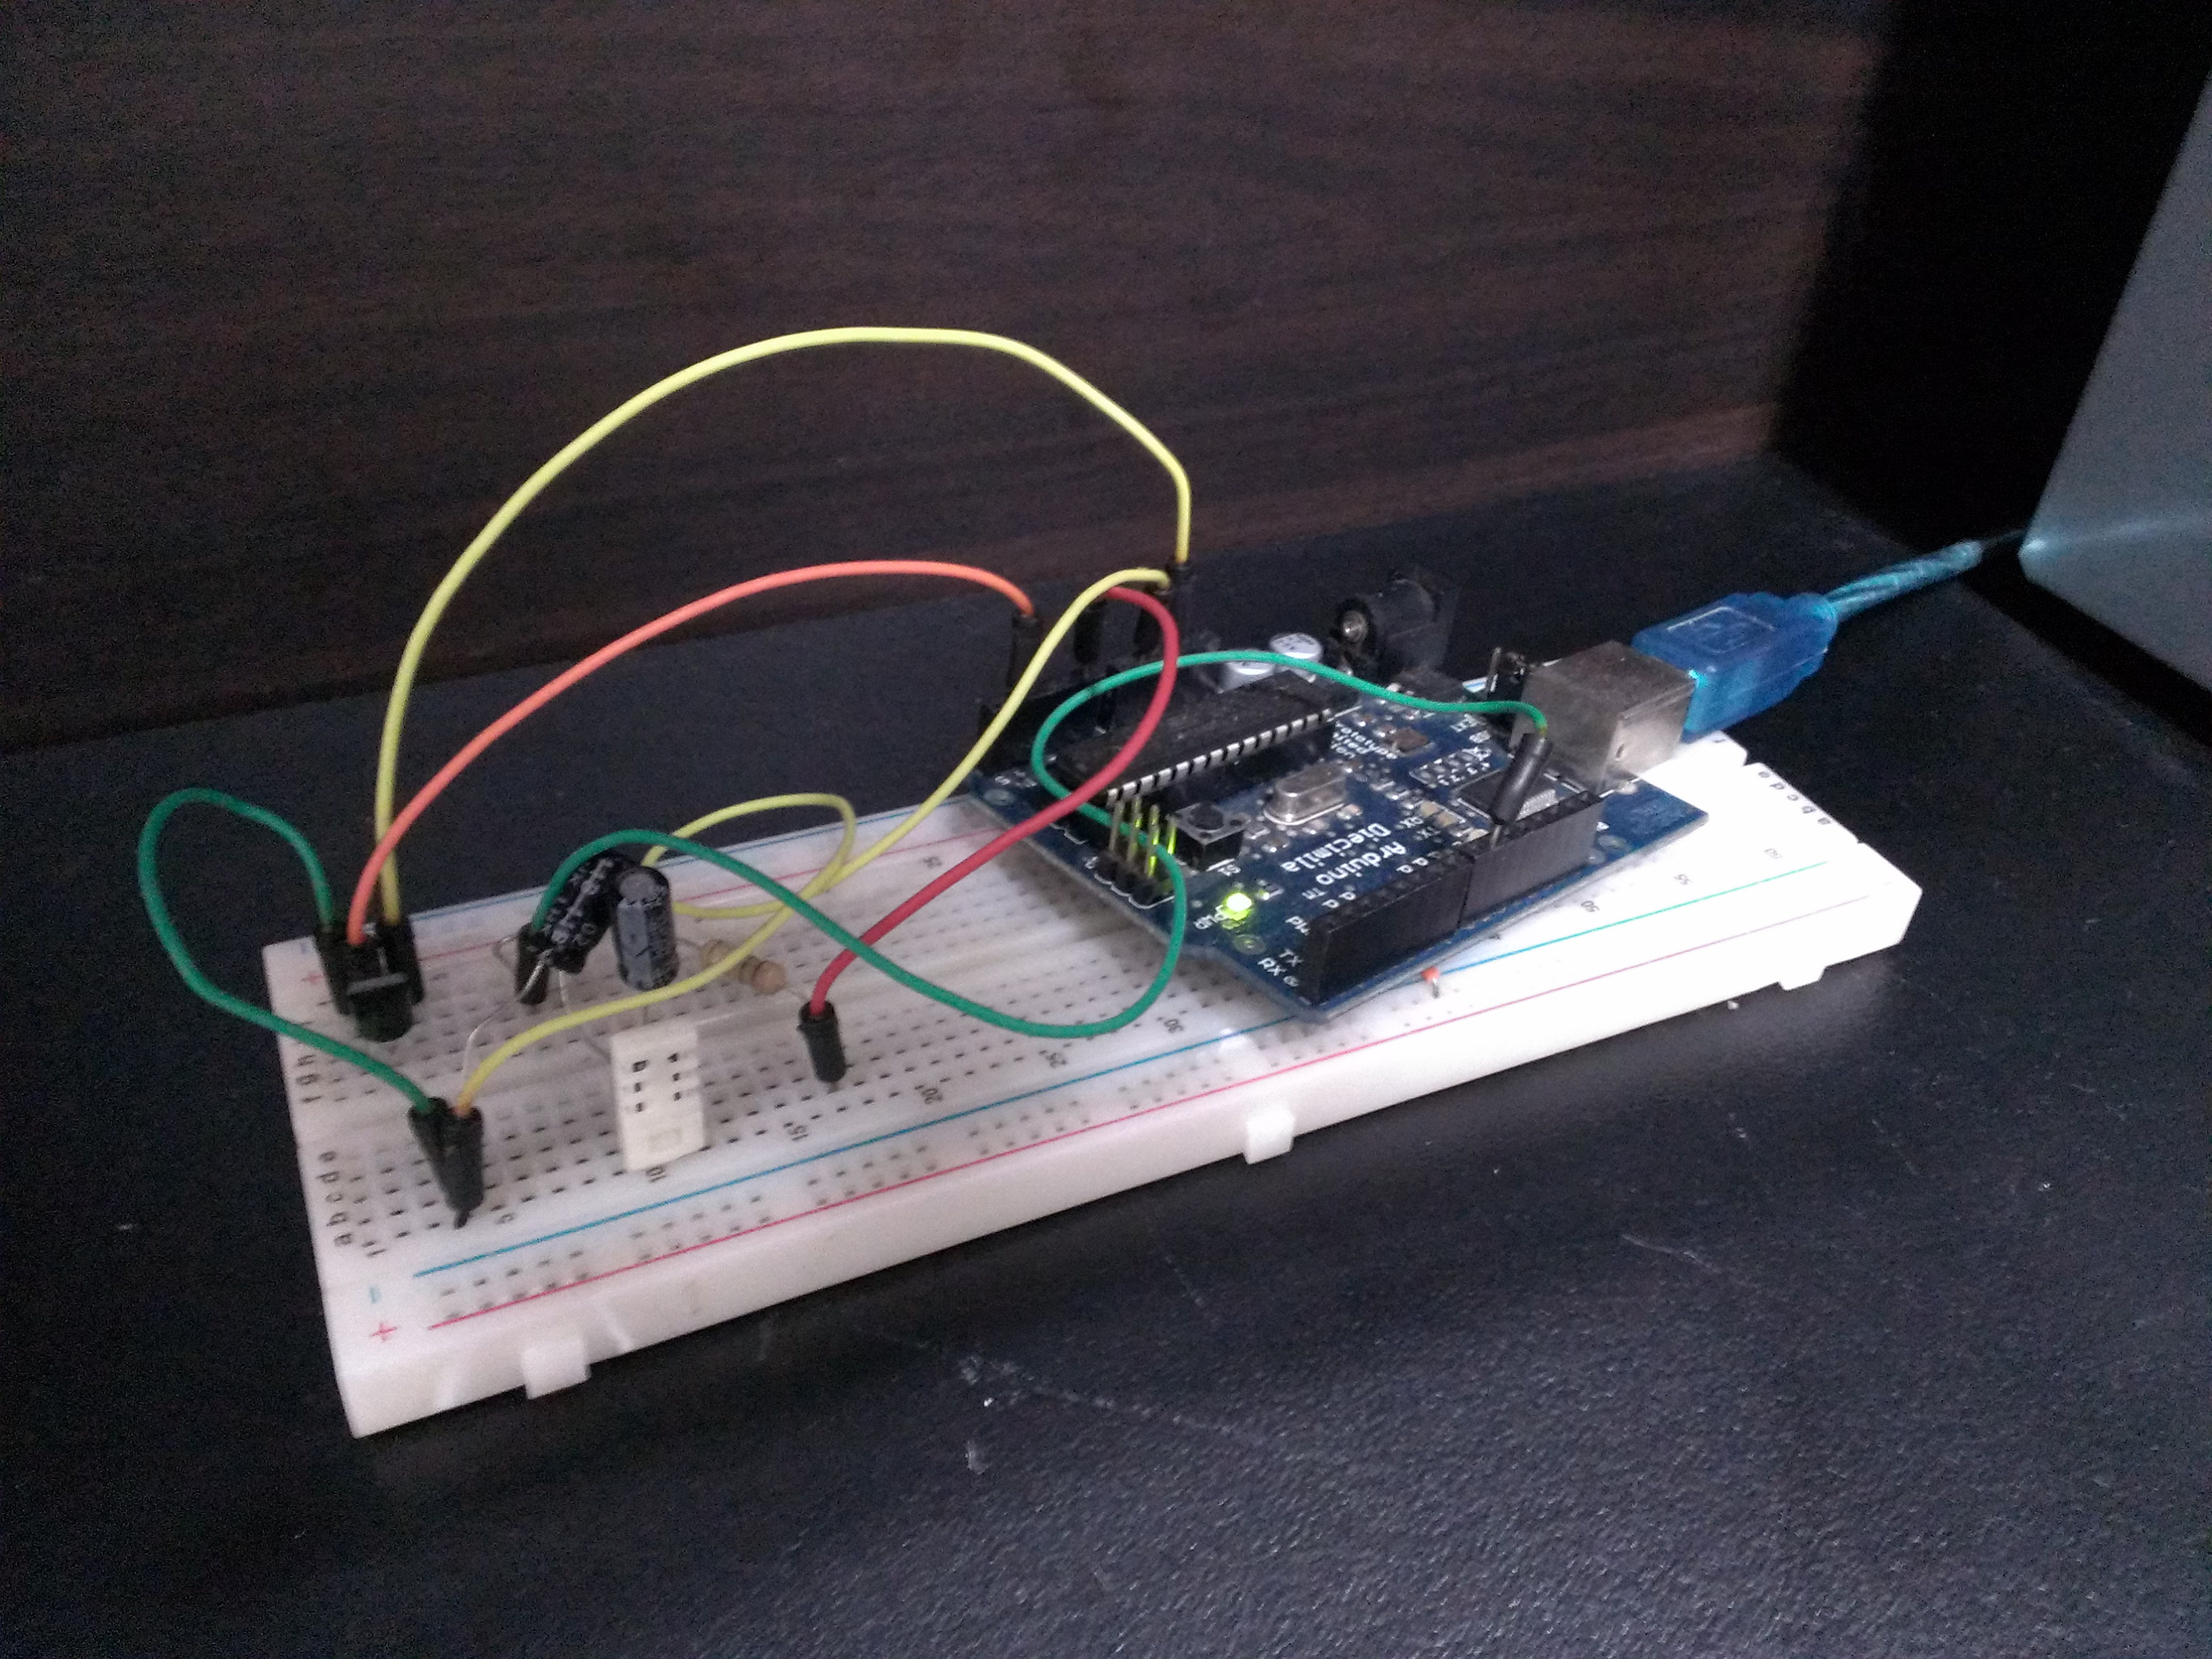
\includegraphics[width=140mm]{setup.jpg}
\caption{The entire setup on the breadboard}
\label{fig:setup}
\end{figure}

\section{Store and display}

On a server computer a Node.js application server gathers the data, displays it on a web interface, and forwards to a database. The source code of that server is on the net\footnote{Server source code: \url{https://github.com/imrehg/weatherstation/tree/master/server}}, and can be installed as it is usual with Node.js applications: install Node.js if not already (tested v0.8.16), download the source, run `npm install` in the source code directory to install the dependencies, create a new configuration file from `config.json.default` into `config.json` (need to add the appropriate MongoDB server information).

The handled data is in JSON format, with 3 fields: `date`, `humidity`, `temperature`.

The current results are available to see on \url{http://hostname:5000/} where `hostname` is the appropriate hostname for the computer running the program.

The database is running MongoDB \, like other monitoring systems for the bakeout, just different database. The recorded weather values are currently kept for 2 weeks set by the appropriate Time-To-Live (TTL) values \footnote{Expiring data: \url{http://docs.mongodb.org/manual/tutorial/expire-data/}}.

\section{Weather report}

The weather report emails are handled by a Python script, that is scheduled to run at regular intervals (once a day). The source code is on the net as well\footnote{Weather report: \url{https://github.com/imrehg/weatherreport}}. Tested with Python 2.7.3.

When installing, a `weather.conf` file has to be created based on `weather.conf.example`, to set the correct configurations for the script.

The running of the script at regular intervals is done by cron (one common scheduler on Linux), have to set the following values in the cron config (with `crontab -e`):
\begin{lstlisting}[language=Bash,frame=single]
0 7 * * * /home/lab/prog/weatherreport/report.sh
\end{lstlisting}
which means that every day, at 7:00am run the following script.

The computer has to be able to send emails with sendmail, another common Linux tool for this to work, and if the dataset has some problems, then might not send email at all (not all error scenarios are foreseen).

\begin{figure}[ht!]
\centering
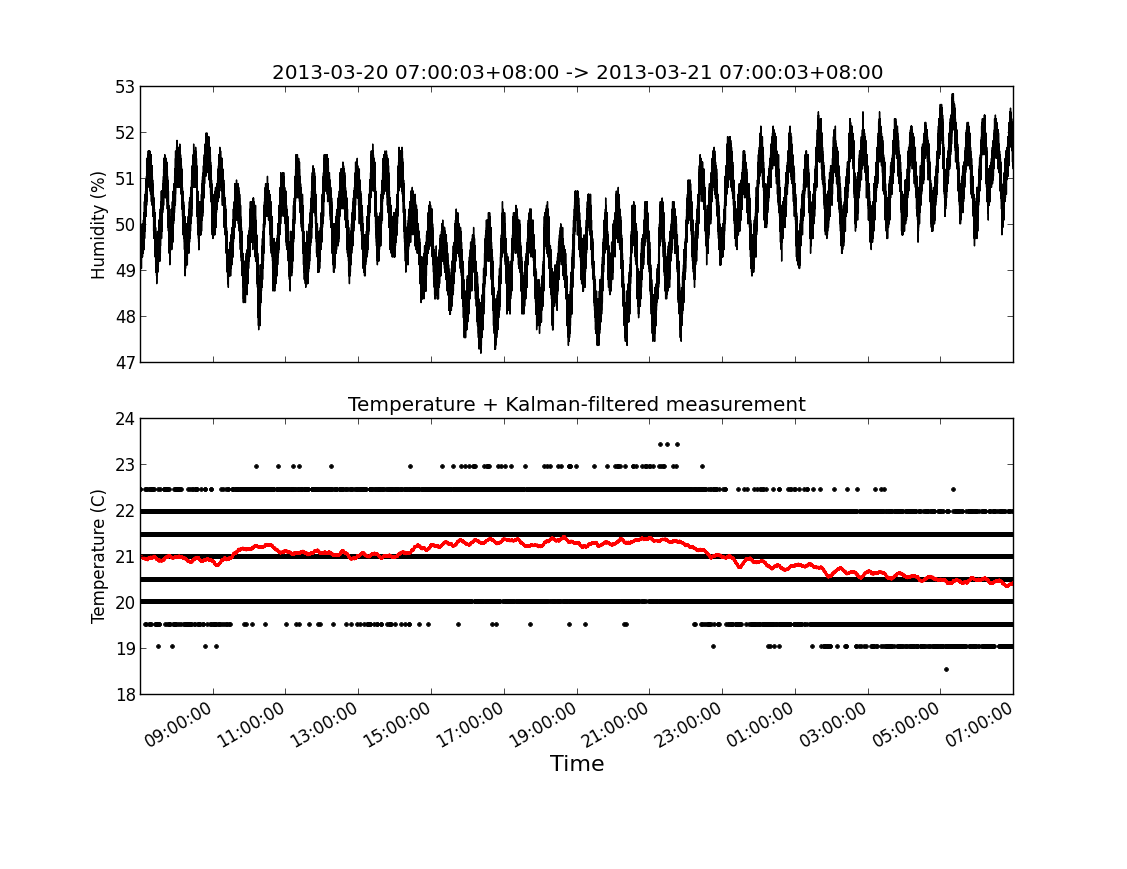
\includegraphics[width=140mm]{20130321-0700.png}
\caption{Example of weather report, for 2013-03-21 07:00:00}
\label{fig:weatherreport}
\end{figure}

%\section{Appendix}
%
%\subsection{Arduino source code}
%\label{ssec:arduino}
%
%\begin{lstlisting}[language=C,frame=single]
%#include <limits.h>  // For ULONG_MAX
%
%static const int VCCPin = 9;
%static const int analogPin = 0;
%static const int tempPin = 4;
%static const float Re = 50.3; // kOhm
%//static const float Vref = 5.0 * 15 / (15 + 51);
%static const float Vref = 5.0;
%static const float Vm = 2.5;
%
%
%static float a = 2.76366367;
%static float b = -32.40924966;
%static float c = 102.93566686;
%
%int val = 0;
%int count = 0;
%unsigned long t;
%boolean level = LOW;
%unsigned long nowt;
%static unsigned long microwait = 500;
%unsigned long deltat;
%
%void setup() {
%  Serial.begin(115200);
%  Serial.println(F("Humidity sensor"));
%  pinMode(VCCPin, OUTPUT);
%  t = micros();
%}
%
%void loop() {
%  float temp, hum, res;
%  
%  nowt = micros();
%  if (nowt >= t) {
%    deltat = nowt - t;
%  } 
%  else {
%    // Taking care of micros overflow
%    // that should happen every 70 minutes or so
%    deltat = ULONG_MAX - t + nowt;
%  }
%  if (deltat > microwait) {
%    digitalWrite(VCCPin, level);
%    if (level == HIGH) {
%      if (count == 400) {
%        res = GetResistance();
%
%        digitalWrite(VCCPin, LOW);
%        delay(50);
%        temp = GetTemperature();
%        digitalWrite(VCCPin, HIGH);
%        
%        hum = GetHumidity(res, temp);
%        Serial.print(hum);
%        Serial.print(",");
%        Serial.print(res);
%        Serial.print(",");
%        Serial.print(temp);
%        Serial.println();
%        count = 0;
%      } else {
%        count++; 
%      }
%    }
%    level = !level;
%    t = nowt;
%  }  
%}
%
%// Output resistance in kOhm
%float GetResistance(void) {
%  float resistance, volt;
%  int val;
%  
%  val = analogRead(analogPin);
%  volt = val * 5.0 / 1024;
%
%  if (volt < Vm) {
%    resistance = -1;
%  } 
%  else if (volt > Vref) {
%    resistance = -2;
%  } 
%  else {
%    // if in range, calculate resistance value
%    resistance = Re / ((Vref-Vm)/(volt-Vm) - 1);
%  }
%  return (resistance); 
%}
%
%// Rewrite these into two functions so can retrive the resistance
%// separately and use temperature to get correct value;
%float GetHumidity(float resistance, float temperature) {
%  float humidity;
%  
%  if (resistance < 0) {
%     // this means there was some error
%     // in the resistance measurement
%     if (resistance == -1) {
%       humidity = 0.0;
%     } else if (resistance == -2) {
%       humidity = 100.0; 
%     } else {
%        humidity = 0.0; 
%     }
%  }
%  else {
%    float reslog = log10(resistance);
%    humidity = a * reslog*reslog + b * reslog + c;
%    if (humidity > 100.0) {
%      humidity = 100.0;
%    } 
%    else if (humidity < 0.0) {
%      humidity = 0.0;
%    }
%  }
%  return (humidity);
%}
%
%float GetTemperature(void) {
%  float temperature;
%  temperature = analogRead(tempPin) * 5.0 / 1024.0 / 0.01;
%  return (temperature);
%}
%\end{lstlisting}

\end{document}